\chapter{Benchmarking and Testing}\label{chp:chp3}

%\begin{flushright}
%%  {\em QUOTE GOES HERE }\\
%
%\ \
%
%\normalsize
%%{AUTHOR}  
%\end{flushright}

There is a general lack of published models in the literature that 
consider dust absorption-affected asymmetric line profiles.  We therefore test 
the code by comparing the results to optically thin profiles that may be 
derived analytically.  We then test the absorption and scattering 
components of the code by comparing our results in the case of an 
optically thick medium with those derived by \citet{Lucy1989} in their 
Model II and Model III scenarios.

\section{Theoretical Line Profiles from First Principles}
\label{analytics}

Analytical profiles may be calculated in the dust-free case.  We ran a 
number of models based on the methods of \cite{Gerasimovic1933} 
who derived equations for line profiles emitted from a transparent 
expanding shell.

\begin{figure}
\begin{subfigure}{0.5\textwidth}
\centering
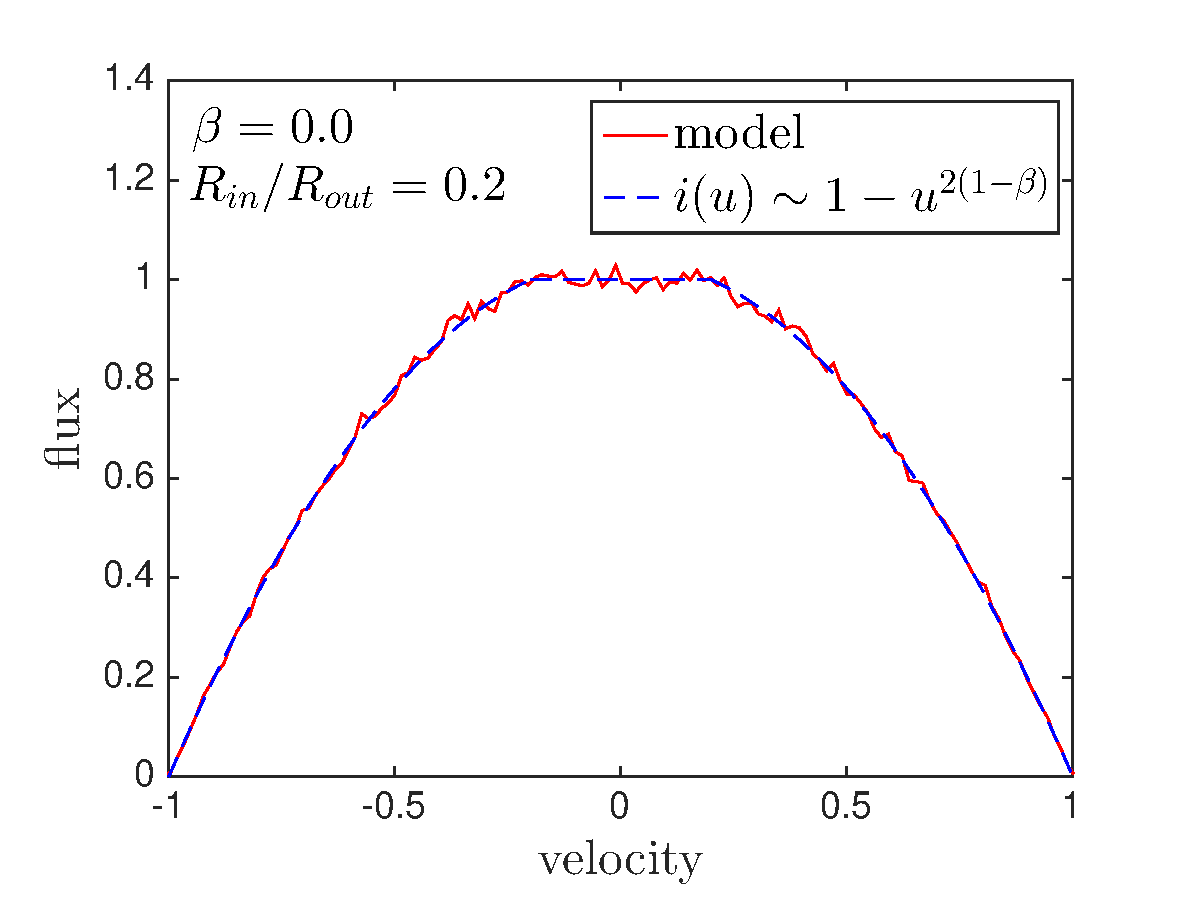
\includegraphics[trim =25 40 45 15,clip=true,scale=0.46]{chapters/chapter4/images/params/A/b0_r0_2}
\end{subfigure}
\hspace{4mm}
\begin{subfigure}{0.5\textwidth}
\centering
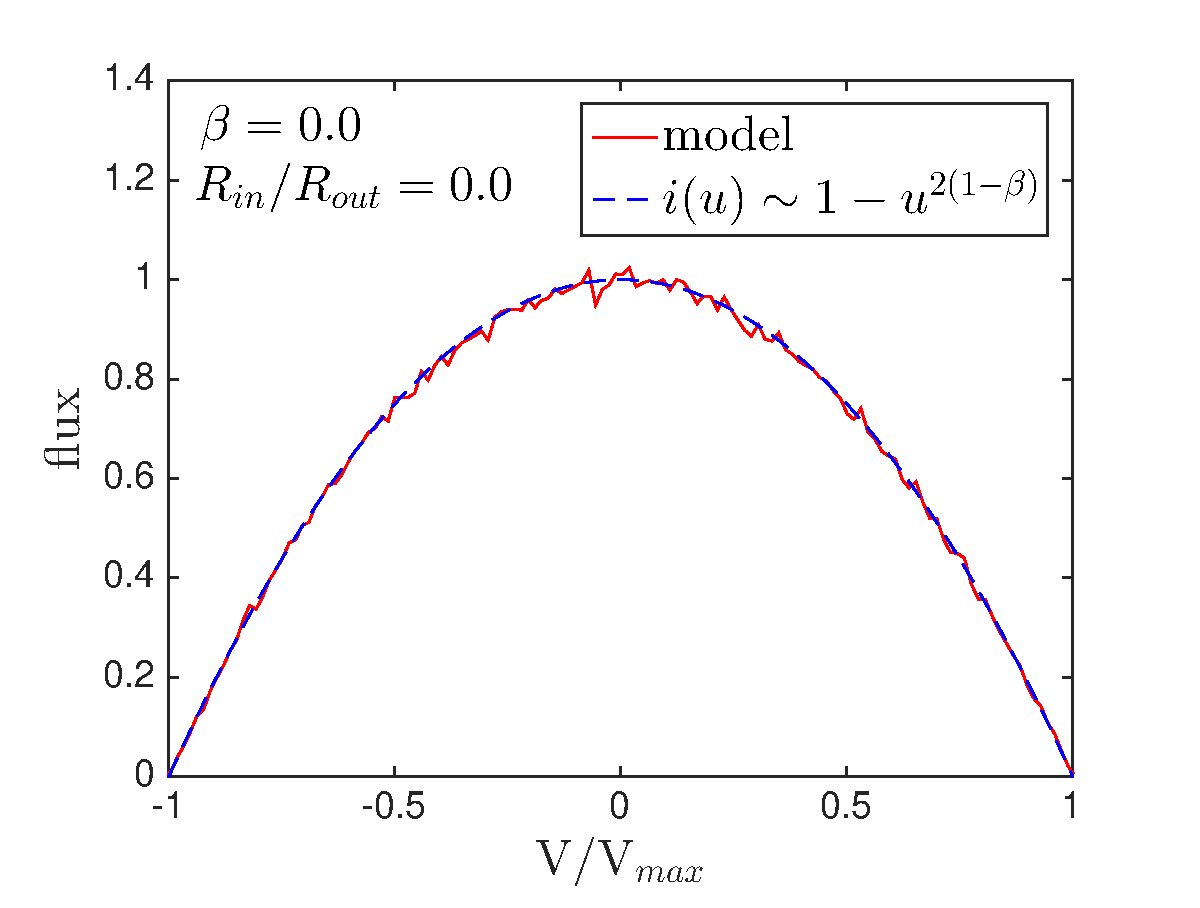
\includegraphics[trim =72 40 45 15,clip=true,scale=0.46]{chapters/chapter4/images/params/A/b0_r0}  
\end{subfigure} \\[0.0ex]

\begin{subfigure}{0.5\textwidth}
\centering
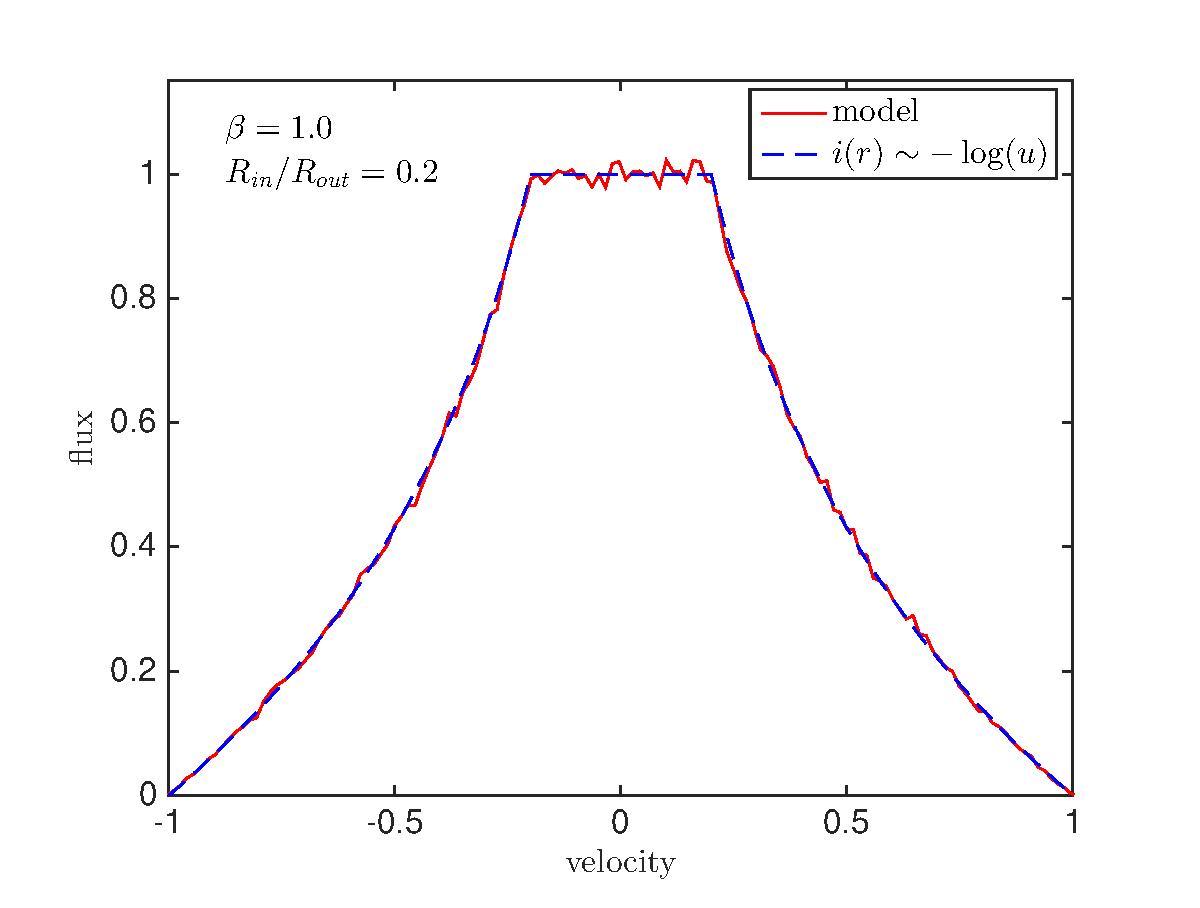
\includegraphics[trim =25 40 45 15,clip=true,scale=0.46]{chapters/chapter4/images/params/A/b1_r0_2}
\end{subfigure}
\hspace{4mm}
\begin{subfigure}{0.5\textwidth}
\centering
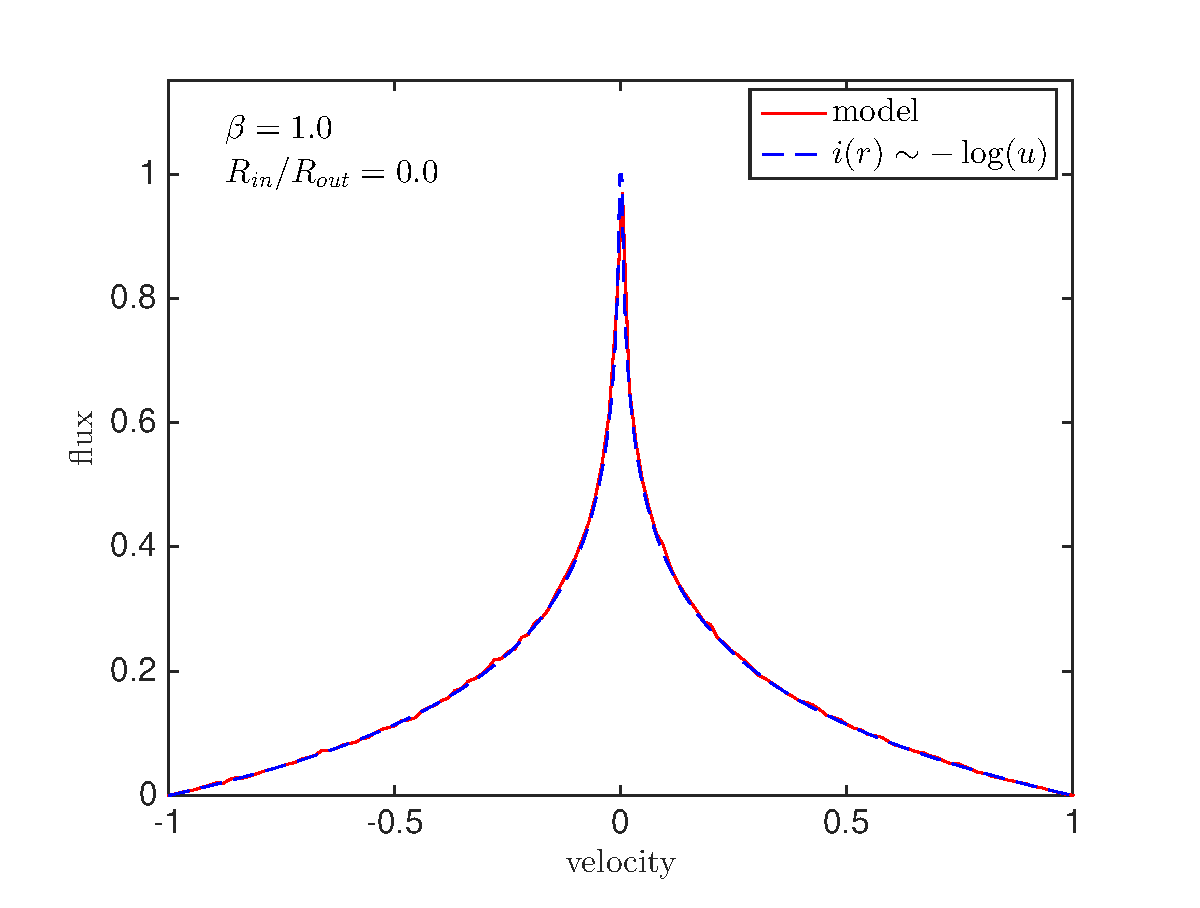
\includegraphics[trim =72 40 45 15,clip=true,scale=0.46]{chapters/chapter4/images/params/A/b1_r0} 
\end{subfigure} \\[0.0ex]

\begin{subfigure}{0.5\textwidth}
\centering
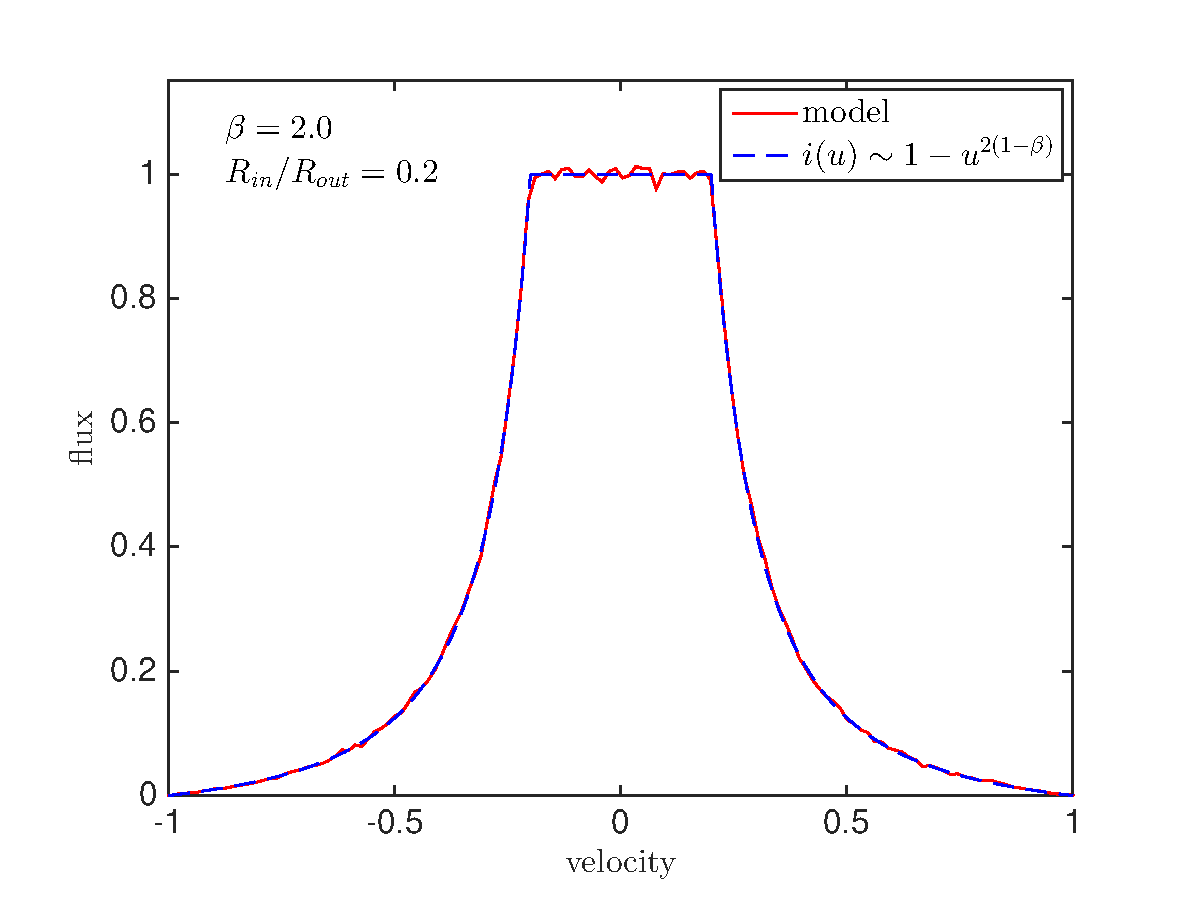
\includegraphics[trim =25 25 45 15,clip=true,scale=0.46]{chapters/chapter4/images/params/A/b2_r0_2}
\end{subfigure}
\hspace{4mm}
\begin{subfigure}{0.5\textwidth}
\centering
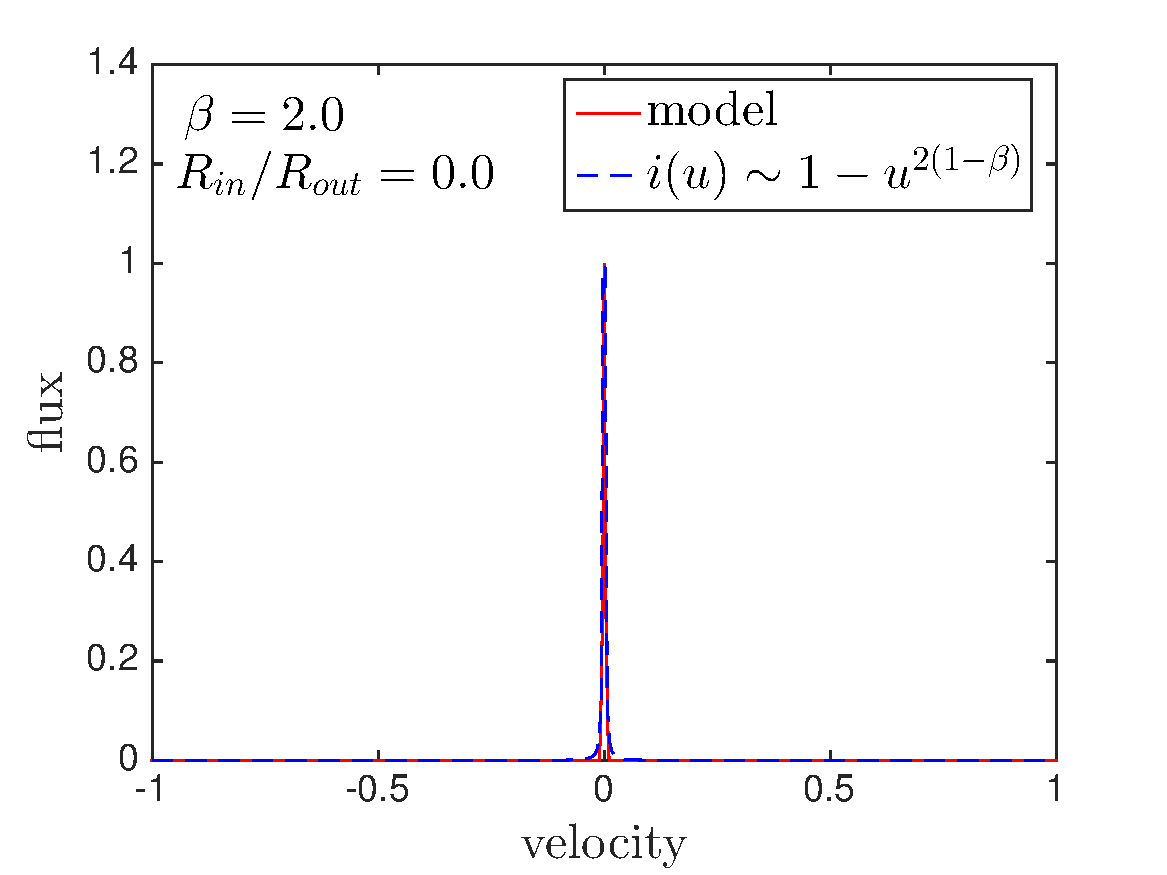
\includegraphics[trim =72 25 45 15,clip=true,scale=0.46]{chapters/chapter4/images/params/A/b2_r0}
\end{subfigure}

\caption{\textit{Red:} Benchmark models for optically thin ($\tau =0$) 
line profiles  with fractional velocity $v \propto r$. Left to right: initial emissivity 
profiles $i(r) \propto r^{-2\beta}$ with $\beta=0.0$, $\beta=1.0$ and 
$\beta=2.0$. Cases with $R_{in}/R_{out}=0.2$ are on the top and 
$R_{in}/R_{out}=0.0$ on the bottom.  The presence of a plateau in the upper plots is due to the finite inner radius (detached shell). \textit{Blue:} The analytical case 
with $i(u) \sim 1-u^{2(1-\beta)}$ except in the case of $\beta=1$ where 
$i(u) \sim -\log u$.}
\label{fig:analytics}
\end{figure}

Describing the fractional expansion velocity of the shell as $v(r)=r^\alpha$ with 
$\alpha \neq 0$ such that $v(r)=\frac{V(r)}{V_{max}}$ where $V(r)$ and $V_max$ represent physical velocities and $v_{max}=1$, the energy emitted by 
the nebula between radial velocities $v$ and $v+dv$ is proportional to

\begin{equation}
\int _\tau i(r) r \sin (\theta) \, r \, d\theta \, dr
\end{equation}

\noindent where $i(r)$ represents the emission per unit volume at radius 
$r$ and $\theta$ is the angle to the observer's line of sight.  We adopt inner radius $R=q$ and outer radius $R=1$.

\begin{figure}
\begin{subfigure}{\textwidth}
\centering
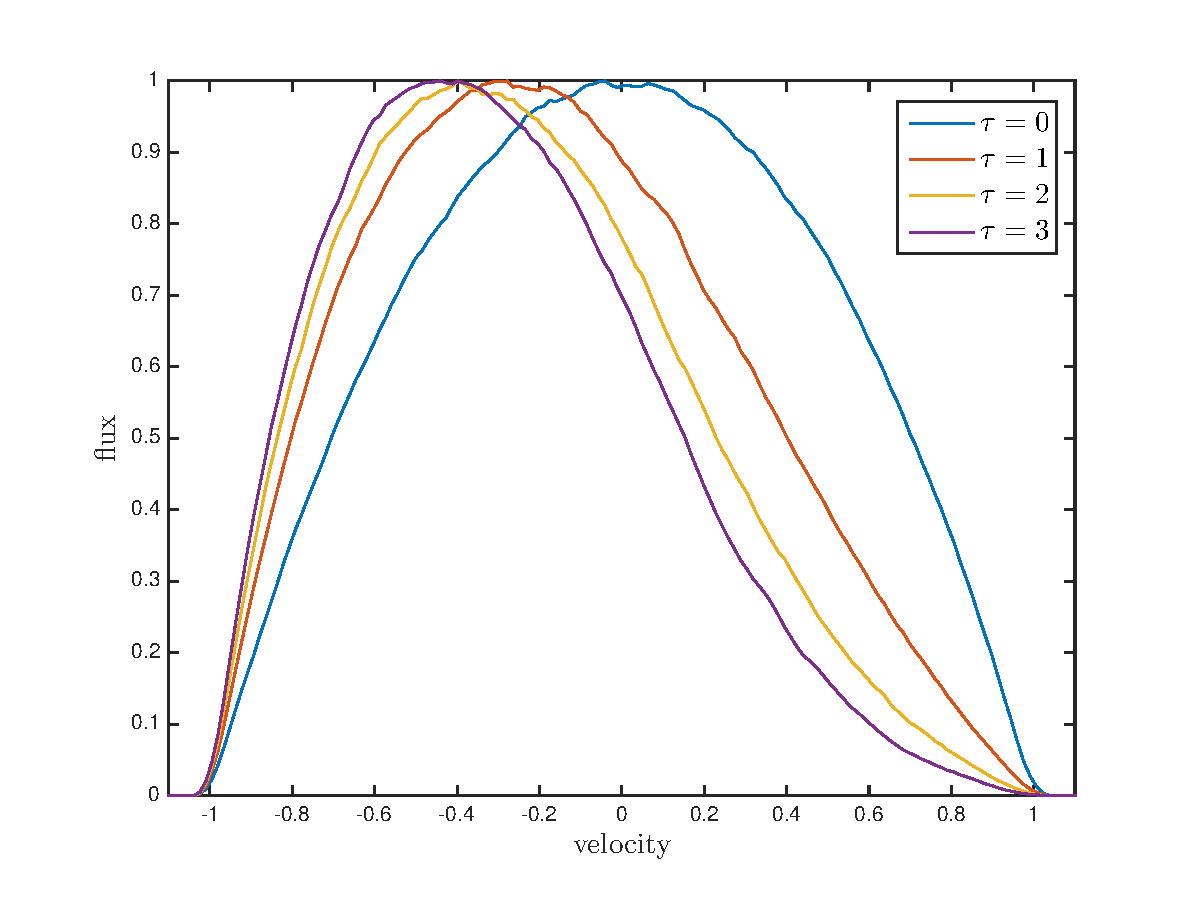
\includegraphics[trim =37 10 45 15,clip=true,scale=0.75]{chapters/chapter4/images/params/opt_thick_w0}
\end{subfigure} \\[1ex]
\begin{subfigure}{\textwidth} 
\centering
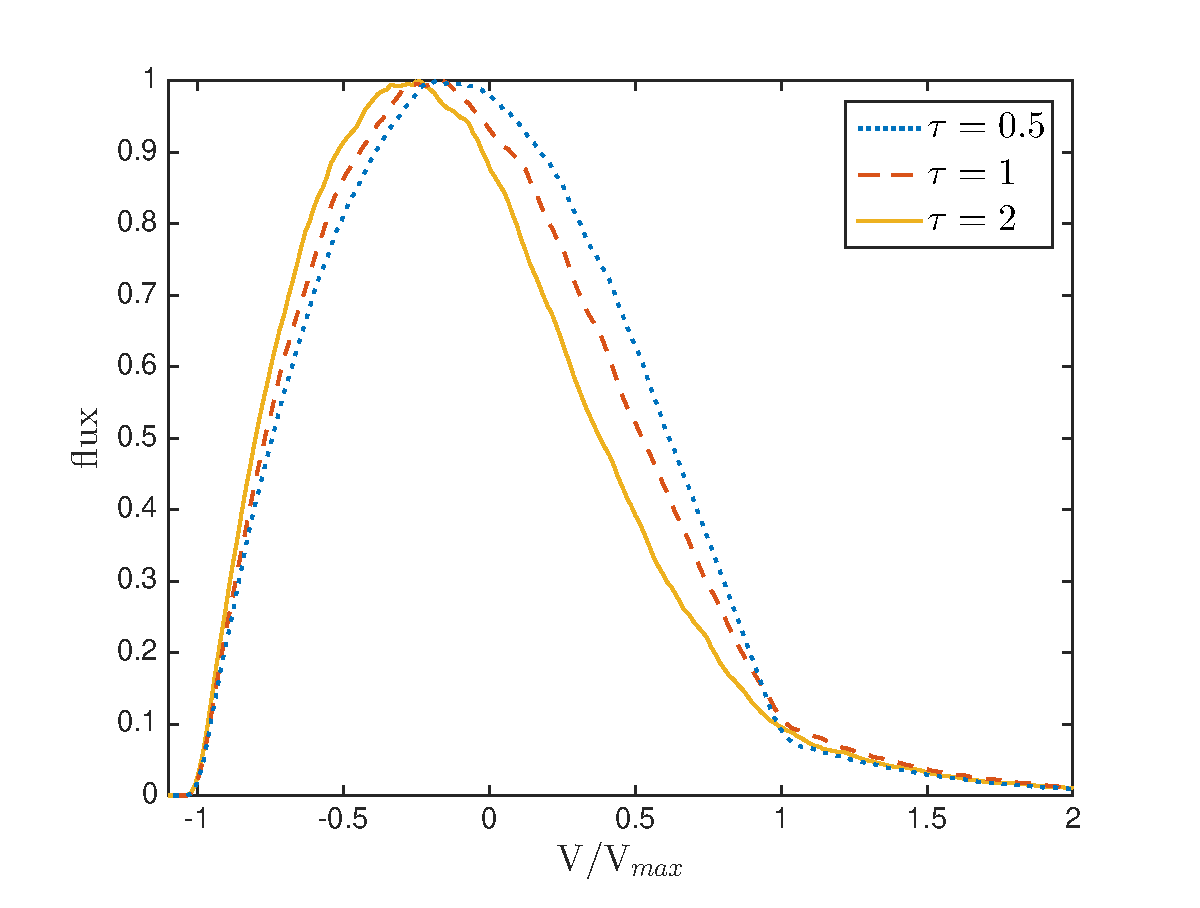
\includegraphics[trim =37 10 45 15,clip=true,scale=0.75]{chapters/chapter4/images/params/opt_thick_w0_6}
\end{subfigure}  
\caption{Benchmark models for line profiles  with $v \propto r$, $i(r) \propto$ constant and a filled sphere with $R_{in}/R_{out}=0$.  Pure dust absorption models ($\omega = 0$) are presented in the top plot, whilst partially scattering models are presented at the bottom ($\omega = 0.6$) as per \citet{Lucy1989} Models II and III. All resulting profiles have been scaled to unity flux at their peaks.}
\label{fig:Lucy}
\end{figure}

Setting $i(r) \propto r^{-2\beta}$ (for a recombination or collisionally excited line emitted from 
a medium with an assumed density profile for the emitter $\rho \propto 
r^{-\beta}$) then gives

\begin{equation}
\begin{split}
i(v) \, dv &\sim \frac{dv}{\alpha v^{\frac{2\beta-3+\alpha}{\alpha}}} \int^{\theta_1}_{\theta_0} \cos^{\frac{2\beta-3}{\alpha}} \theta \sin \theta \, d\theta 
\\
&\sim  \frac{dv}{v^{\frac{2\beta-3+\alpha}{\alpha}}} \Bigg[\frac{\cos^{\frac{2\beta - 3 + \alpha}{\alpha}} \theta}{2\beta -3 + \alpha}\Bigg]^{\theta_1}_{\theta_0}
\end{split}
\end{equation}

\noindent for $\frac{2\beta-3}{\alpha} \neq -1$ where $i(v) \,dv$ is the energy emitted in a volume element and $\theta_0$ and $\theta_1$ are the bounds of this element.  The case 
$\frac{2\beta-3}{\alpha} = -1$ results in a logarithmic relationship.



In the case of a ``complete'' nebula, i.e. one where the inner radius is 
vanishingly small in comparison to the outer radius, we obtain

\begin{equation}
\label{eqn:sides}
	i(v) \, dv \sim \pm \frac{du}{(2\beta-3+\alpha) v^{\frac{2\beta-1+\alpha}{\alpha}}} \Big(1-v^{\frac{2\beta-3+\alpha}{\alpha}} \Big)
\end{equation}

If the nebula is not ``complete'', that is to say, the inner radius is some fraction of the outer radius and the remnant is a detached shell, the above formula becomes valid only from $v=1$ to some critical value $v'=q^\alpha$. For $v<v'$, we obtain

\begin{equation}
i(v) \, dv \sim \pm \frac{dv}{(2\beta-3+\alpha)} \Big( \frac{1}{q^\alpha} - 1 \Big)
\end{equation}

\noindent and therefore the top of the line is flat while the sides are 
sloping.

Crucially, the width of the flat section is determined by $v'=q^\alpha$ or 
simply $v'=q$ in the case where $v \propto r$, whilst the shape of the 
profile outside of the flattop is described by equation \ref{eqn:sides}.

Profiles with a variety of shapes may be derived from these formulae 
depending on the relative values of $\alpha$ and $\beta$.  Here we 
consider three main families of curves:


%\begin{minipage}{0.55\textwidth}
\begin{enumerate}\parskip3pt

	\item \ \ $\quad i(v)  \sim v^{-\gamma}-1$ \quad ($\alpha>0$, $2\beta-3+\alpha>0$)
	\item \ $\quad i(v)  \sim 1-v^\gamma$ \quad \ \ ($\alpha>0$, $2\beta-3+\alpha<0$)
	\item  $\quad i(v) \sim -\log v$ \quad \ \ ($\alpha>0$, $2\beta-3+\alpha=0$)

\end{enumerate}
%\end{minipage}


\noindent where $\gamma$ is defined as $\gamma= \lvert 
\frac{2\beta-3+\alpha}{\alpha} \rvert$.

Models are presented for each of these cases, both for a 
complete nebula and for a shell structure with $R_{in}/R_{out}=0.2$.  
A velocity profile $v \propto r$ appropriate for supernova ejecta in the free 
expansion phase is used throughout.  Values of $\beta = 0, 1$ and $2$ are 
adopted.  Figure \ref{fig:analytics} illustrates the excellent agreement between 
the analytical case and the models.  All fluxes are scaled to unity at the peak.

\section{The Line Profile Models of \citet{Lucy1989}}
\label{opt_thick_testing}

In addition to the tests for optically thin lines described above, we also 
compared our outputs to those derived by \citet{Lucy1989} in order to 
assess the accuracy of the scattering and absorption aspects of the code.  
We consider two similar cases, equivalent to Models II and III of 
\citet{Lucy1989}. In the first case, dust with zero albedo is 
uniformly distributed throughout a completely filled nebula with a velocity profile 
$v \propto r$.  In the second case, the same scenario is considered but a 
medium of dust with albedo $\omega =0.6$ is considered.

In the first case, the profile may once again be derived analytically from 
the basic geometry using the fact that radiation will be attenuated by a 
factor $e^{-2\tau_{\nu} v}$ between points with line of sight fractional velocities $-v$ and 
$+v$ where $\tau_{\nu}$ is optical depth at frequency $\nu$ from the centre to the outer edge of the ejecta.  The line profile is therefore given by

\begin{equation}
\frac{I(v)}{I(-v)} = \exp(-2\tau_{\nu} v)  
\end{equation}

\citet{Lucy1989} presented several examples for both the analytical case of 
the perfect absorber and a Monte Carlo model for grains with $\omega 
=0.6$.  We present the same cases in Figure \ref{fig:Lucy} and note that 
the resulting profiles exhibit the same features and shape. Of particular 
interest is the scattering wing that appears beyond the maximum velocity 
($v_{max}=1$) on the red side of profiles in the case of the partial 
scatterer, as a result of the packets doing work on the expanding sphere.  
This was noted by \citet{Lucy1989} as a potential diagnostic for the 
presence of dust in the ejecta of a supernova and we will discuss this 
further in Section \ref{ps}.

\section{Testing the Electron Scattering Mechanism}
%\section{Clumped models in smooth limits}


